\subsection{Query Graph Generation}
\label{sec:candgen}

%We start introducing our KBQA system from candidate generation step.
%Given a complex question,
%it's a common practice to generate all possible query graphs through
%multiple stages~\cite{yih2015semantic,bao2016constraint}.
%Intuitively, the generation process begins from
%extracting candidate focus nodes in the question using linking tools.
%Then we connect the answer node to the corresponding focus entity
%using predicate sequences in KB.
%We call it ``main path'' and it is the basis of more complex structures.
%Further, we attempt to attach more constraints to the main path,
%%which are represented predicate sequences connect the remaining focus nodes to the main path,
%leading to complex query graphs in a tree shape.
%%The main intuition is to first find focus entities as the starting point of all candidate structures,
%%then extract main paths, and finally enrich the main path by adding different kinds of constraints.
We illustrate our staged candidate generation method in this section.
% While this method is similar with \citet{bao2016constraint},
% we mainly discuss the main differences between ours and theirs.
Compared to previous methods, such as \citet{bao2016constraint}, we employ a more effective candidate
generation strategy, which takes advantage of implicit type information in query graphs
and time interval information in the KB.
%and we mainly discuss our differences.
%we make improvements.
%In our candidate generation process,
%different semantic constraints to the answer set 
%The constraints that we can handle
In our work, we take 4 kinds of semantic constraints into account:
\textbf{entity}, \textbf{type}, \textbf{time} and \textbf{ordinal} constraints.
\figref{fig:candgen} shows a concrete example of our candidate generation.
%Now we begin to explain in details the different candidate generation stages.
For simplicity of discussion, we assume Freebase as the KB in this section.
%by performing SPARQL querys : generate main path first, and enrich add different kinds of constaints.
%Given a question, we    multiple stages.  (follow Bao and Yih)
%(need two detail figures showing the different parts)


\begin{figure*}
	\centering
	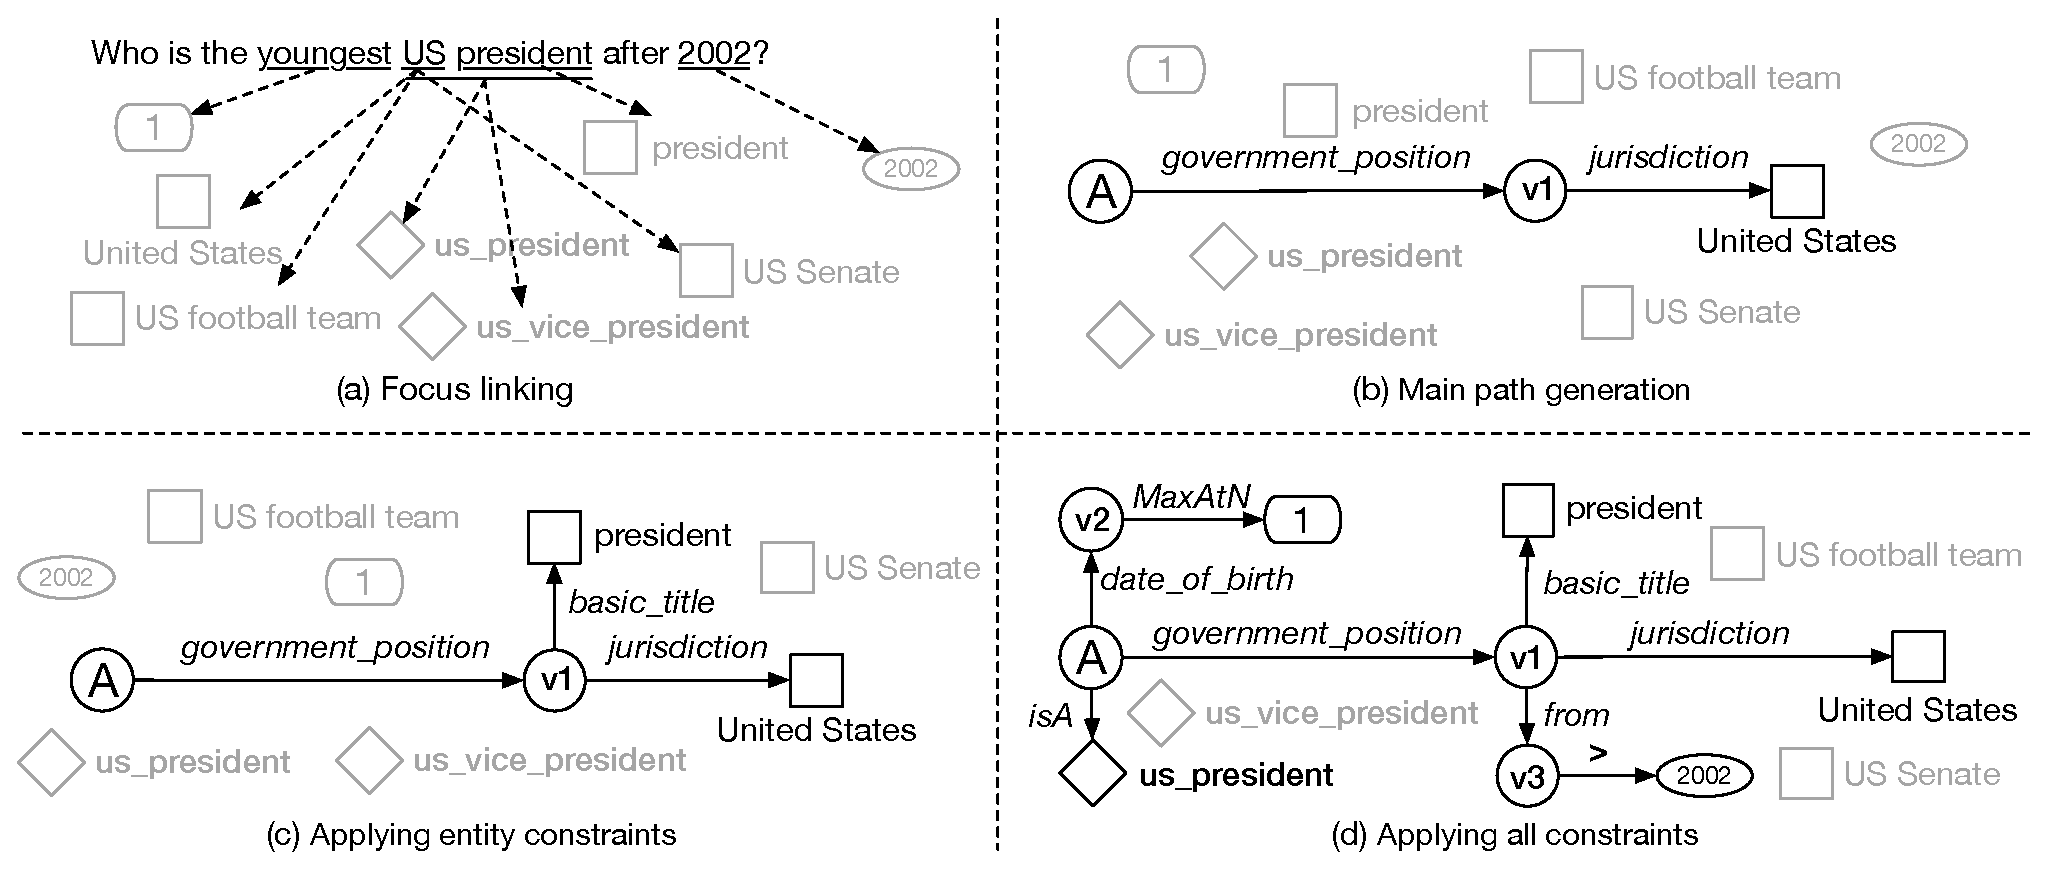
\epsfig{file=figures/cangen.eps, angle=0, width=2.0\columnwidth}
	%\scalebox{0.3}{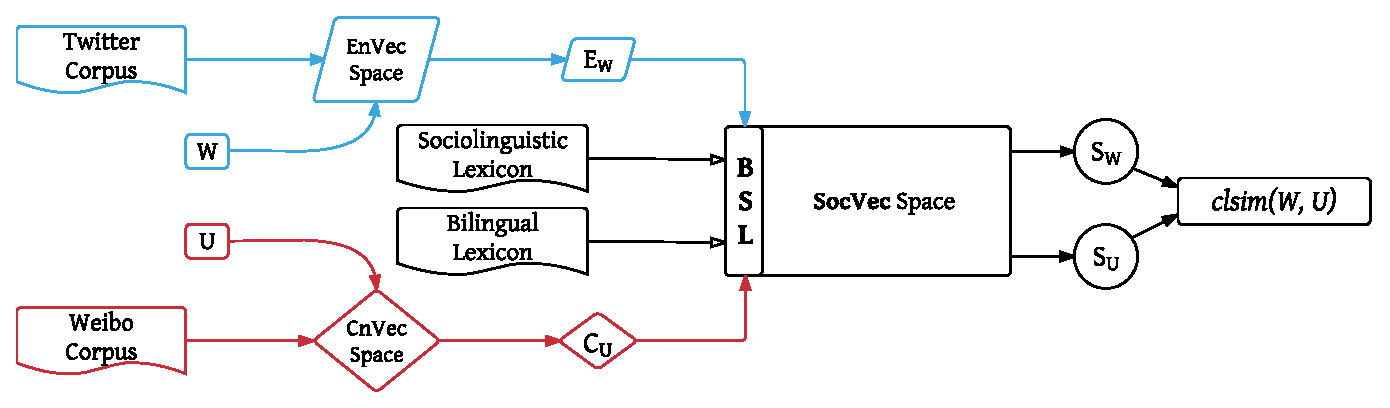
\includegraphics{overview.eps}}
	\caption{Running example of candidate generation.}
	\label{fig:candgen}
\end{figure*}


%TODO: "who is the youngest president of the united states after 2002 ?"
%TODO: draw the graph, make simpler predicate names.

\textbf{Step 1: Focus linking.}
%This step takes the question as input, and returns candidate (mention, focus) pairs,
%where focus node 
%for example, (``United State'', \textit{united\_states})
We extract possible (mention, focus node) pairs from the question.
%We extract possible focus mentions (words or phrases in the question)
%and link them to nodes in KB or literal values.
Focus nodes are the starting points of various semantic constraints,
refer to \figref{fig:candgen}(a).
%for example in \figref{fig:candgen}(a),
%we link ``US'' to the entity \textit{united\_states},
%or ``US president'' to the type \textit{us\_president}.
%Different linking methods are used for different categories of focus nodes.
%For entity linking, we adopt a state-of-the-art linking tool, S-MART~\cite{yang2015s},
%which is widely used in previous KBQA researches.
%it scores candidate (mention, entity) pairs based on statistical features from Wikipedia,
%such as the lexical similarity, link probability and entity popularity.
%The output is a list of (mention, entity) with linking scores,
%and one mention can link to multiple entities.
For entity linking, we generate (mention, entity) pairs
using the state-of-the-art entity linking tool S-MART~\cite{yang2015s}.
%trained on Twitter corpus.
%Following the S-MART results provided by Yih et al.~\shortcite{yih2015},
%up to 10 top-ranked (mention, entity) pairs will be returned.
%One mention could lead to several entities.
%For example, the mention ``Star Trek'' links to several possible films in the result.
For type linking,
%due to the limited number of types in Freebase,
%we propose a simple but effective method for extracting (mention, type) pairs.
%we perform an embedding based brute force search.
we brutally combine each type with all uni-, bi- and tri-gram mentions in the question,
and pick top-10 (mention, type) pairs with the highest
word embedding similarities of each pair.
%we enumerate all uni-, bi- and tri-gram mentions of the question,
%and calculate the cosine similarities of averaging word embeddings
%between the mention and all the type names.
%Top-10 scoring (mention, type) pairs are kept as type linking results.
%and pair them with all the types in Freebase.
%For each (mention, type) pair, we calculate the cosine similarity
%of averaging word embedding vectors between them,
%and keep top-10 scoring pairs as type linking results.
For time linking, we extract time mentions by simply matching year regex.
For ordinal linking, we leverage a predefined superlative word list\footnote{
\texttildelow 20 superlative words, such as largest, highest, latest.}
and recognize mentions by matching superlative words,
or the ``ordinal number + superlative'' pattern.
%``superlative'', ``ordinal number + superlative'' or ``superlative + adjective''.
The ordinal node is an integer representing the ordinal number in the mention.
%For example, we retrieve (``youngest'', 1) in \figref{fig:candgen}(a).


\textbf{Step 2: Main path generation.}
%The most simple query graph is a predicate sequence from
%the answer node to a focus entity,
%since all factoid questions are related to at least one entity in the question.
%We call it ``main path'', since it's the basis of more complex structures.
%We first build coarse query graphs by using focus entities only, since almost all factoid questions
%are related to at least one entity (except corner cases like ``Who's the fastest man in the world?'').
%The output of this step is refer to \figref{fig:candgen},
%where: one ore more entities are linked to the answer entity by FB predicates in a tree shape.
%For constructure different tree shapes,
We build different main paths by connecting the answer node to different focus entities
using 1-hop or 2-hop-with-mediator\footnote{
Mediator is a kind of auxiliary nodes in Freebase maintaining N-ary facts.}
predicate sequence.
\figref{fig:candgen}(b) shows one of the main paths.
Further constraints are attached by
%In the perspective of query graphs, a constraint is represented as a predicate sequence
connecting an anchor node $x$ to an unused focus node through predicate sequences,
where the anchor node $x$ is a non-focus node in the main path
($A$ or $v_1$ in the example).

\textbf{Step 3: Attaching entity constraints.}
%In this step, 
We apply a depth-first search to search for combinations of
multiple entity constraints to the main path through 1-hop predicate.
\figref{fig:candgen}(c) shows a valid entity constraint, ($v_1, basic\_title, president$).
The advantage of depth-first search is that we can involve unlimited number of entities
in a query graph, which has a better coverage than template-based methods.
%Fuzzy SPARQL queries are applied 
%for quickly finding all valid predicates between an anchor node and a focus entity,
%SPARQL query over Freebase all combination of predicates with certain shape.
%Compare with template based generation, our adv is to involve multiple entities 
%are generate query graphs in a flexible way.

%Given all possible focus entitie of the question, we first build the main path of the query structure.
%We enumerate each entity as the main entity, and take the regard remaining as possible contraint entities.
%We search the knowledge base and explore all 1-hop and 2-hop-with-med predicate sequences
%starting from the main entity.
%For example, ...
%along this path, answer node could be xxxx and the intermediate entity are mediators describing the particular actor-film-starring fact.
%Afterwards, we attempt to add entity constraints to the main paths.
%%TODO: add SPARQL query example to the query structure
%if the constraint entity can be linked to the answer entity or intermediate entity by some 1-hop predicates.
%As the running example of Figure xxx, the constraint entity yyy is connected to the entity by the predicate "zzz".

\textbf{Step 4: Type constraint generation.}
Type constraints can only be applied at the answer node using \textit{IsA} predicate.
%that is, connecting the answer node to existing focus types through \textit{type.object.type} predicate in Freebase.
%Meanwhile,  we can infer implicit types of the answer node based on its outgoing predicates.
%For example, we infer that answers have the type \textit{politician} by knowing that
%``\textit{government\_position} is the predicate of \textit{politician} in Freebase''.
Our improvement in this step is to filter type constraints
using \textbf{implicit types} of the answer, derived from the outgoing predicates 
of the answer node.
For example in \figref{fig:candgen}(c), 
the domain type of the predicate \textit{government\_position}
is \textit{politician}, which becomes the implicit type of the answer.
Thus we can filter type constraints which are irrelevant to the implicit types,
preventing semantic drift and speeding up the generation process.
%Different from previous methods, in order to prevent semantic drifting, 
%we consider the implicit types of the answer, derived by
%the outgoing predicates of the answer.
%For example in \figref{fig:candgen}(c),
%we infer the implicit type \textit{politician} by knowing that
%\textit{government\_position} is the predicate of \textit{politician} in Freebase.
To judge whether two types in Freebase are relevant or not,
we adopt the method in \citet{luo2015inferring} to build a rich type hierarchy of Freebase.
Focus types are discarded, if they are not the super- or sub- types
of any implicit types of the answer.
%type subsumption relation in Freebase, and discard those focus types,
%if they are not the super or sub types of any implicit types of the answer.
%we allow a focus type if it's the super or sub type of 
%if the focus type is the super or sub type of any implicit types.
%For building subsumption relationship between Freebase types,
%we adopt the method proposed by \citet{luo2015inferring} which considers soft set inclusion.

%Type constraint is more restricted, where a candidate FB type is linked to only the answer node by ``type.object.type'' in FB.
%Since S-MART doesn't provide information of type mentions, we propose a simple but effective method for detecting type mentions.
%In order to make the query structure consistent in semantics, we attempt to apply the type
%constriant to the current query structure, if there are overlapping s between the type
%and the range type of the main path.
%Taking xx as example, the range is ``location'', therefore candidate type like ``river'' can be applied,
%non-overlapping candidate types (like ``person'', ``book'') are discarded, if existed.
%TODO: Talk about topical consistent predicates.

\textbf{Step 5: Time and ordinal constraint generation.}
As shown in \figref{fig:candgen}(d), the time constraint is represented
as a 2-hop predicate sequence, 
%where the first is the KB predicate which points to a time,
where the second is a virtual predicate determined by the preposition before the focus time,
indicating the time comparing operation, like ``before'', ``after'' and ``in''.
Similarly, the ordinal constraint also forms a 2-hop predicate sequence,
where the second predicate represents descending (\textit{MaxAtN}) 
or ascending order (\textit{MinAtN}).

For the detail of time constraint,
while existing approaches \cite{yih2015semantic,bao2016constraint} 
link the focus time with only single time predicate,
our improvement is to leverage \textbf{paired time predicates}
for representing a more accurate time constraint.
%Suppose we are generating time constraints for the phrase ``in 2002'',
In Freebase, paired time predicates are used to represent facts within certain time intervals,
like $from$ and $to$\footnote{
Short for $governmental\_position\_held.from$ and $governmental\_position\_held.to$
respectively.} in \figref{fig:candgen}(d). 
For time comparing operation ``in'', we link the time focus to the starting time predicate,
but use both predicates in SPARQL query,
restricting that the focus time lies in the time interval of the paired predicates.
%Time constraint is a bit different from previous constraints: 
%the semantics is largely related to the
%preposition before the focus time, like ``before'', ``after'' and ``in''.
%Thus the predicate sequence in time constraint is 2-hop,
%where the second predicate represents the direction of time comparison
%and is determined by the particular preposition, refer to the predicate ``$>$''
%in \figref{fig:candgen}(d).
%Besides, time related facts are usually described with twin predicates,
%indicating the start and end time, respectively.
%When translating a query graph into SPARQL language,
%we leverage both predicates to verify whether answer entities satisfy time constraints,
%like ``in 2002''.
%Thus we extract predicates pointing to integer, float or datetime values,
%and then concatenate with each order predicate, resulting in ordinal constraints.
%Without a clear evidence of choosing which one, we generate ordinal constraints
%for both orders, 
%As shown in \figref{fig:candgen}(d), one possible ordinal constraint
%is to sort answer entities by \textit{date\_of\_birth}, and pick the largest one.

%Time constraint is similar with entity constraint, where 
%focus time can be linked to variables in the main path.
%
%we enumerate time predicate of under implicit types and attach.
%a little bit different:
%triple with comparisons (y, xxx, > 2010)
%Besides,
%In FB, time information are usually described by two predicates, indicating the start and end time.
%For example, blabla versus balbla.
%So we actually link two edges, as shown in \figref{xxx}.

%We extract time mention by simply matching year regex.
%Different from the previous constraints, the preposition before the time mention is meaningful,
%then we include it into the time mention.
%Then we attampt to link the time to main paths through the "op+predicate" sequence.
%the predicate is inplicit datetime predicates of the 
%intermediate entity and answer node (including constraint types binding to the answer).
%The preposition represents datetime comparison operators as lt, gt, within.

%\textbf{Ordinal}
%Similar with time constraint: finding mentions and link throught "op+predicate" sequence.
%mention: ordinal words (``fist'', ``2nd'') and superlative words (``longest'', ``largest'').
%We collect the set of superlative words which tends to describe factual and object attributes.
%Therefore, the mention encodes both target ranks and the semantic of ordinal predicates.
%The op are chosen from two virtual operators: max and min.
%The predicate are topical consistent predicates whose range are int, float or datetime.
%in order to control the size of cands brought by ordinal constraints,
%leverage word embedding ,extract top-2 by calculating the cosine similarity
%between mention embedding and predicate name embedding.

After finishing all these querying stages,
we translate candidate graphs into SPARQL query, and produce their final output answers.
Finally, we discard query graphs with zero outputs, or using overlapped mentions.
%In summary, the candidate generation method is inspired by \citet{bao2016constraint},


%in summary, inspired by Yih, Bao: Fewer rules, and consider time interval.


%Given a question, we have to generate a set of query graphs with multiple complex constraints. In general, we first detect entities mentioned in the question. Then for each entity, we regard it as a fixed node and starting from it we search for a path in KB. A path is composed of at most two hop predicates. For example, the $\bi{sk}_1$ in the right part of \figref{fig:overview} is such a path with one hop predicate since ``China'' is an entity.

%However, basic path can only express the semantics of single relation question, but can not support a question with multiple complex constraints such as the one in \figref{fig:overview}. Thus, we have to add those complex constraints to the simple path to restrict the answer. There are four different constraints in our consideration, which are entity constraint, type constraint, temporal constraint and ordinal constraint. Entity constraint, 




